\begin{frame}{Uncertainty in Event Detection}
\begin{figure}
    \centering
    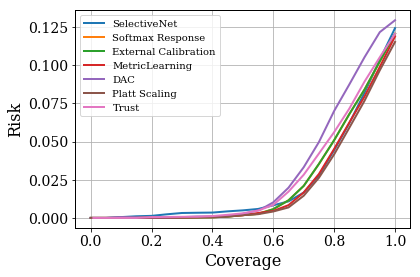
\includegraphics[width=0.5\textwidth]{Problem2/figures/Calibration_riskCoverage.png}    
\end{figure}
Coverage is defined as the percentage of data remaining after churning out documents on which the model score is less than the identified threshold. 

The curve is plotted by first sorting the model predictions in terms of its confidence score and moving the threshold from 0 to 100th percentile value of the confidence score. 

\end{frame}